% Lecture Template for ME3001-001-Tristan Hill - Spring 2020
% Mechanical Engineering Analysis with MATLAB
%Numerical Integration - Lecture 3

% I am finally converting my stuff to BEAMER
% and I am putting these on Github because Dropbox is defective

% Document settings



%\documentclass{beamer}                  % for presentation ?
\documentclass[handout]{beamer}  % for handout ?
\usepackage{beamerthemesplit}
\usepackage{amsmath}
\usepackage{listings}
\usepackage{multicol}
\usepackage{framed}

\usepackage{soul}


\beamertemplateballitem

\definecolor{TTUpurple}{rgb}{0.3098, 0.1607, 0.5176} % TTU Purple (primary)
\definecolor{TTUgold}{rgb}{1.0000, 0.8666, 0.0000} % TTU Gold (primary)

\setbeamercolor{palette primary}{bg=TTUpurple,fg=TTUgold}
\setbeamercolor{palette secondary}{bg=black,fg=TTUgold}
\setbeamercolor{palette tertiary}{bg=black,fg=TTUpurple}
\setbeamercolor{palette quaternary}{bg=TTUgold,fg=black}
\setbeamercolor{structure}{fg=TTUpurple} % itemize, enumerate, etc
\setbeamercolor{section in toc}{fg=TTUpurple} % TOC sections

%\usefonttheme{professionalfonts}

%

\newcommand{\vspccc}{\vspace{6mm}\\} % large vertical space
\newcommand{\vspcc}{\vspace{4mm}\\}   % medium vertical space
\newcommand{\vspc}{\vspace{2mm}\\}     % small vertical space

\newcommand{\hspcccc}{\hspace{10mm}} % large horizontal space
\newcommand{\hspccc}{\hspace{6mm}} % large horizontal space
\newcommand{\hspcc}{\hspace{4mm}}   % medium horizontal space
\newcommand{\hspc}{\hspace{2mm}}     % small horizontal space

\newcommand{\paramM}{100} % mass, m
\newcommand{\paramC}{0.5}  % drag coeff, c
\newcommand{\paramVO}{5.0} % initial velocity, v0
\newcommand{\paramDTA}{1.0} % timestep, dt  - A
\newcommand{\paramDTB}{0.1} % timestep, dt  - B
\newcommand{\paramDTC}{0.01} % timestep, dt  - C


\newcommand{\LNUM}{2\hspace{2mm}} % Lecture Number 
\newcommand{\secondtitle}{Solving Higher-Order Equations with ODE45}% second line of the title of this  presentation , aka the topic of this lecture

\title{\vspace{2mm}\\Numerical Integration - Lecture \LNUM}
\author{ME3001 - Mechanical Engineering Analysis} % original formatting from Mike Renfro, September 21, 2004

\date{April 17, 2020}

\begin{document}

\lstset{language=MATLAB,basicstyle=\ttfamily\small,showstringspaces=false}


% Section 0 - Outline (I know there is a beamer thing for this...)
\frame{\titlepage \center\textbf{\secondtitle}\vspcc}

\frame{

{\bf Lecture \LNUM - \secondtitle :} \vspace{3mm}\\ % ' topics' are beamer 'sections' - TWH

\begin{multicols}{2}

\includegraphics[scale=0.15]{baxter.jpg}\vspc

\large
 \begin{itemize}

	\item Review ODE45 Function\vspace{4mm}\\
	\item A More Exciting Model \vspace{4mm}\\
	\item Equation Decomposition  \vspace{4mm}\\	
	\item MATLAB Solution\vspace{4mm}\\

\end{itemize}
%\includegraphics[scale=0.4]{euler01.jpg}\vspc
%\small Leonard Euler (1707-1783)
\end{multicols}
}

% Section 1 - Review ODE45 function

\subsection{Using the ODE45 function}

\frame[containsverbatim]{

  \frametitle{Using the ODE45 function}

 
The {\bf ode45} function is a powerful tool and it is easy to use. \vspace{0mm}\\

  \begin{lstlisting}

[t_45,y_45]=ode45(@ODEFUN,TSPAN,Y0,OPTIONS,P...);
 
  \end{lstlisting}

\vspace{3mm} Here is a description of the arguments.\vspace{2mm}\\

ODEFUN - name of the function containing the model \vspace{2mm}\\
TSPAN - time range for the initial value problem \vspace{2mm}\\
Y0 - initial value of the dependent variable \vspace{2mm}\\
OPTIONS - options defined by OPTIMSET function \vspace{2mm}\\
P... - additional parameters passed to ODEFUN \vspace{2mm}\\


}

\subsection{Euler's Method in MATLAB}
\frame[containsverbatim]{
  \frametitle{Euler's Method in MATLAB}

 \begin{lstlisting}
% approximate with Euler's forward integration
v_eu(1)=v0;
for j=1:length(time)-1
    v_eu(j+1)=v_eu(j)+f(time(j),v_eu(j),m,c)*dt;  
end

% If this is an 'Inline Definition' of the function 
% it MUST go at the bottom of the script
function [dvdt]=f(t,v,M,C)
    dvdt=-C/M*v;
end

  \end{lstlisting}

}

% Section 2 - A More Exciting Model
\section{A More Exciting Model}
\subsection{A More Exciting Model}
\frame{

\frametitle{A More Exciting Model}
\begin{itemize}

\item First and second order linear models are frequently used  in science and engineering

\item However the world is \underline{\hspace{15mm}-\hspace{40mm}}\\

\item Many exciting and important engineering problems invlove {\bf more complex models} involving rotational motion.

\end{itemize}

\includegraphics[scale=0.15]{ur5e.png}
\includegraphics[scale=0.25]{dji_phantom.jpg}
\includegraphics[scale=0.07]{steady_cam.jpg}

}

\frame{

\frametitle{Non-Linear Swinging Pendulum}

An example of a non-linear system is an {\it inverted pendulum metronome}. \vspc

\begin{multicols}{2}
\includegraphics[scale=0.15]{metronome.png}

How will this system behave?\vspc
\scalebox{1}{$I_o\ddot{\theta}+k_T-\left( m\cdot g\cdot l\right) sin(\theta)=0$} \vspcc

Finding an analytical solution is {\bf very involved} and only mathematicians have time for all that...but you can look \href{https://www.researchgate.net/publication/230969993_A_comprehensive_analytical_solution_of_the_nonlinear_pendulum}{\color{blue}here\color{black}}

\end{multicols}

}

% Section 3 - Equation Decomposition
\section{Equation Decomposition}
\subsection{Equation Decomposition}
\frame{
As we have seen using Euler's method is not hard, but we have to setup the problem correctly. This is a re-occuring theme! \vspccc
\scalebox{1}{$I_o\ddot{\theta}+k_T-\left( m\cdot g\cdot l\right) sin(\theta)=0$} \vspcc

To solve a second order system with an integration method like Euler's you must write the {\bf slope function(s)}. \vspccc

There are two derivatives so there are two \underline{\hspace{15mm}}\hspace{3mm}\underline{\hspace{20mm}}. \vspc

}


\subsection{x2 First Order from x1 Second Order}
\frame{

\frametitle{x2 First Order from x1 Second Order}

{\it One} second order ODE can be {\bf decomposed} into {\it two} first order ODEs through a simple change of variables. This step can be confusing, but remember it is just an algebraic substitution!\vspccc

	\scalebox{1}{$I_o\ddot{\theta}+k_T-\left( m\cdot g\cdot l\right) sin(\theta)=0$} \vspcc

}


\subsection{Execute Euler's Method}
\frame{

\frametitle{Execute Euler's Method}
\scalebox{1.0}{$f_1=$}\vspc
\scalebox{1.0}{$f_2=$}\vspc
Use Euler's method just as before with both slope functions. Compute the values of the solution one-by-one {\bf forward in time} for each variable side-by-side. \vspcc
\begin{tabular}{|c|c|c|}\hline
i&\scalebox{0.7}{$z_1(t_{i+1})=z_1(t_i)+f_1(t_i,z_{1i},z_{2i})\Delta t$}&\scalebox{0.7}{$z_2(t_{i+1})=z_2(t_i)+f_2(t_i,z_{1i},z_{2i})\Delta t$}\\ \hline
1&\scalebox{0.7}{$z_1(\hspccc)=z_1(\hspccc)+f_1(\hspccc,\hspccc,\hspccc)\Delta t$}&\scalebox{0.7}{$z_2(\hspccc)=z_2(\hspccc)+f_2(\hspccc,\hspccc,\hspccc)\Delta t$}\\ \hline
2&\scalebox{0.7}{$z_1(\hspccc)=z_1(\hspccc)+f_1(\hspccc,\hspccc,\hspccc)\Delta t$}&\scalebox{0.7}{$z_2(\hspccc)=z_2(\hspccc)+f_2(\hspccc,\hspccc,\hspccc)\Delta t$}\\ \hline
3&\scalebox{0.7}{$z_1(\hspccc)=z_1(\hspccc)+f_1(\hspccc,\hspccc,\hspccc)\Delta t$}&\scalebox{0.7}{$z_2(\hspccc)=z_2(\hspccc)+f_3(\hspccc,\hspccc,\hspccc)\Delta t$}\\ \hline
\end{tabular}

\vspace{5mm} As you can see this can get messy quickly. 




}



% Section 4: MATLAB Solution
\section{MATLAB Solution}

\subsection{Part 1 - Program Setup}
\frame[containsverbatim]{
  \frametitle{Part 1 - Program Setup}



\begin{lstlisting}

clear variables;close all;clc

% define the constant parameters
global m g l kt; % global variables, gross...
m=2;g=9.8;
l=42*(1/100);kt=6;

% initial conditions
theta0=15;
omega0=0;

% create an array of time values
dt=.001;tstop=10;
time=0:dt:tstop;
\end{lstlisting}

}

\subsection{Part 2 - Euler's Method}
\frame[containsverbatim]{
  \frametitle{Part 2 - Euler's Method}

% This method is not suitable for manual computation. \vspace{0mm}\\

 \begin{lstlisting}
z1(1)=theta0*pi/180; z2(1)=0;  % initial conditions
			 
for j=1:length(time)-1  % approximate with Euler's
    z1(j+1)=z1(j)+f1(time(j),z1(j),z2(j))*dt;  
    z2(j+1)=z2(j)+f2(time(j),z1(j),z2(j))*dt;
end

function [z1dot]=f1(t,Z1,Z2)  % fns. go at bottom
    global m g l kt % even grosser
    z1dot=Z2;
end

function [z2dot]=f2(t,Z1,Z2)
    global m g l kt 
    z2dot=(m*g*l*sin(Z1)-kt*Z1)/(m*l^2);
end
  \end{lstlisting}

}

\subsection{Part 3 - Graph the Solutions}
\frame[containsverbatim]{
  \frametitle{Part 3 - Graph the Solutions}

% This method is not suitable for manual computation. \vspace{0mm}\\

 \begin{lstlisting}
% plot the results of the method
figure(1);hold on
plot(time,z1,'r')
plot(time,z2,'b')
grid on
title('Non-Linear Pendulum')
legend('Angular Pos. (rad)','Angular Vel. (rad/s)')
xlabel('Time(s)')
axis([0 tstop -3 3])
  \end{lstlisting}

}


\frame[containsverbatim]{
\frametitle{ Do you believe the results?}

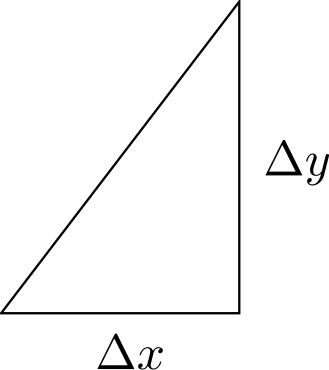
\includegraphics[scale=0.3]{lecture2_fig2.png} \includegraphics[scale=0.3]{lecture2_fig3.png}  \\
\small This graph on the left makes sense, but what about this on the right?
}


\end{document}









